%\documentclass[compress,dvips,xcolor=table]{beamer}
\usepackage{etex}
%\documentclass{article}
%\usepackage{beamerarticle}
%\usepackage[turkish]{babel}
\usepackage{tikz}
\usetikzlibrary{shapes,arrows,positioning,calc,shadows,matrix,fit}
\usepackage{pgf-umlcd}
\tikzstyle{umlcolor}=[color=\umldrawcolor,fill=\umlfillcolor,text=\umltextcolor,drop shadow]
\usepackage[utf8]{inputenc}
\usepackage{listings}
\usepackage{multicol}
%\includeonlyframes{current}

\def\circtxt#1{$\mathalpha \bigcirc \mkern-13mu \mathtt #1$}
\def\NO{{\color{red!60!black}$\times$}}
\def\OK{{\color{green!60!black}$\surd$}}

\mode<article>
{
  \usepackage{fullpage}
  \usepackage{pgf}
  \usepackage{hyperref}
}

\mode<presentation>
{
  \usetheme{metuceng}

%  \setbeamercovered{transparent}
}


\title{Programming Language Concepts}
\subtitle{Object Oriented Prog: Objects}
\author{Onur Tolga Şehitoğlu}
\institute[ODTÜ]{Bilgisayar Mühendisliği}
\subject{Object Oriented Prog: Objects}
\date{}
	\titlegraphic{\insertmetutitle\insertlicense}


\begin{document}
\lstset{language=C,
        basicstyle=\scriptsize\ttfamily,
        keywordstyle=\color{blue!50!black}\bfseries,
        identifierstyle=\color{blue!60!green}\sffamily,
        stringstyle=\color{red!70!green}\ttfamily,
	commentstyle=\color{blue!30!white}\itshape,
        showstringspaces=true}
\setbeamercolor{hexample}{bg=green!5!white,fg=black}%
\setbeamercolor{cexample}{bg=blue!5!white,fg=black}%
\setbeamercolor{pexample}{bg=orange!5!white,fg=black}%
\setbeamercolor{oexample}{bg=violet!5!white,fg=black}%

 \frame[plain]{\maketitle}
 \begin{frame}
 \frametitle{Outline}
 \begin{multicols}{2}
 \tableofcontents
 \end{multicols}
 \end{frame}

\section{Object Oriented Programming}
\begin{frame}
\frametitle{Object Oriented Programming}
\begin{itemize}
\item Abstraction
\item Encapsulation
\item Hiding
\item Inheritance
\end{itemize}
\end{frame}

\begin{frame}
\frametitle{Encapsulation/Scope}
\begin{columns}
\begin{column}{8cm}
\begin{itemize}
\item Objects consist of:
\begin{itemize}
\item attributes (member variables)
\item methods (member functions)
\end{itemize}
encapsulated in a package scope
\end{itemize}
\end{column}
\begin{column}{4cm}
\scriptsize
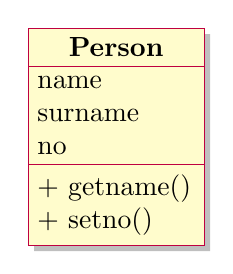
\begin{tikzpicture}
\begin{class}[text width=2cm]{Person}{0,0}
    \attribute{name} 
    \attribute{surname}
    \attribute{no}
    \operation{+ getname()}
    \operation{+ setno()}
\end{class}
\end{tikzpicture}
\end{column}
\end{columns}
\begin{itemize}
\item attributes: state of objects
\item methods: behaviour of objects
\item alternative terminalogy: messages\\
	call a method $\equiv$ send message to an object
\item A class is the family for similar objects. 
\item An object is an \structure{instance} of a class.
\end{itemize}
\end{frame}

\defverbatim[colored]\codePerson{
\begin{lstlisting}[language={C++},escapechar=\#]
class Person {
    char name[40], surname[40];
    int no;
public:
    const char * getname() { return name;}
    void setno(int);
} obj ;

void Person::setno(int a) {
    no=a;
}
\end{lstlisting}}
\begin{frame}
\begin{beamercolorbox}{cexample}
\codePerson
\end{beamercolorbox}
\begin{itemize}
\item C++ allows definitions inside the class or outside by \structure{scope operator `::'}
\item Environment is recursive collateral.
\item \lstinline!obj.getname();! calls the method in the context of object \texttt{obj}.
\item \lstinline!this! keyword denotes pointer to current object in member functions.
	(\lstinline!self()! in some other languages)
\end{itemize}
\end{frame}

\begin{frame}
\frametitle{Hiding}
\begin{itemize}
\item Interface vs detail. Details are hidden, only interface members are exported outside.
\item C++ uses \lstinline!private:, protected:,! and \lstinline!public:! labels to mark hiding.
\item only members following a \lstinline!public:! label are visible outside (the object for
example). Member functions can access all members regardless of their labels.
\item \lstinline!obj.setno(4)! is legal, \lstinline!obj.no! is not.
\item Hiding depends on scope and it is lexical. In C++ pointer conversions can violate hiding.
\item By convention all member variables should be private, some member functions
	can be private, only some of member functions are public.
\item \lstinline!protected! keyword is useful with inheritance.
\end{itemize}
\end{frame}

\begin{frame}
\frametitle{Abstraction}
\begin{itemize}
\item An object is an abstraction over the programming entity defined by the model in the
design.
\item Model: customer, bank, registration, course, advisor, mail, chatroom,...
\item Class should provide:
\begin{itemize}
\item Transparent behaviour for the objects, access via interface functions.
\item Data integrity. Objects should be valid through their lifetimes.
\end{itemize}
\item Data integrity at the beginning of lifetime provided by constructors (+destructors in C++)
\end{itemize}
\end{frame}

\defverbatim[colored]\codePersoncons{
\begin{lstlisting}[language={C++},escapechar=\#]
class Person {
    char *name[40], *surname[40];
    int no;
public:
    Person(const char *n, const char *s) {
         strcpy(name,n) ; strcpy(surname,s) ; no=0;
    }
    Person() { name[0]=0; surname[0]=0; no=0;}
} obj ;
\end{lstlisting}}
\section{Constructors/Destructors}
\subsection{Constructors}
\begin{frame}
\frametitle{Constructors}
\begin{itemize}
\item Special member functions called when lifetime of the object starts
	\alert{just after storage of members are ready}
\item Automatically called. No explicit calls.
\item no return value, name is same with the class
\item can be overloaded
\begin{beamercolorbox}{cexample}
\codePersoncons
\end{beamercolorbox}
\end{itemize}
\end{frame}

\begin{frame}
\begin{itemize}
\item Constructors can be overloaded\\ {\scriptsize
	\begin{tabular}{>{\tt}l>{\tt}l}
	\bf Definition & \bf Constructor \\ \hline
	Person a ; & Person() \\
	Person a("ali","veli"); & Person(const char *, const char *) \\
	Number a=3; & Number(int) \\
	Number a(3); & Number(int) \\
	Number b=a; & Number(Number \&a) \\
	Number a[2]=\{0,1\} & Number(int) \\
	\end{tabular}}
\item If no constructor implemented, empty constructor (do nothing) assumed
\item If at least one constructor exists, variables should match at least one of them,
	no empty constructor assumed
\item Constructors are called by the language when lifetime started:\\
\begin{enumerate}
\item	start of program for global objects
\item	entrance to function for local objects
\item   when heap objects are created (with \lstinline!new!)
\end{enumerate}

\end{itemize}
\end{frame}

\subsection{Heap Objects}
\begin{frame}
\frametitle{Heap Objects}
\begin{itemize}
\item \lstinline!new! and \lstinline!delete! operators
	instead of \texttt{malloc()} and \texttt{free()}. Why?
\item \lstinline!Person *p=new Person("ali","veli");!\\
	\lstinline!delete p;!
\item Array allocation/deallocation:\\
	\lstinline!Person *p=new Person[100];!\\
	\lstinline!delete [] p;!
\end{itemize}
\end{frame}

\subsection{Destructors}
\begin{frame}
\frametitle{Destructors}
\begin{itemize}
\item When storage (members) of an object allocated dynamically
\item Lifetime is over : garbage
\item We need calls to collect heap variables within the object
\item Java solution: garbage collector does the job. We need nothing
\item C++: \structure{destructors}: member functions called when lifetime
	is over.
\item A class only have one destructor with exact type and name: \lstinline!\~ClassName()!.
	Called:
\begin{enumerate}
\item	end of program for global objects
\item	return from function for local objects
\item   when heap objects are deallocated (with \lstinline!delete!)
\end{enumerate}
\end{itemize}
\end{frame}

\subsection{Constructor Calls}
\begin{frame}
\frametitle{Constructor Calls}
\begin{itemize}
\item Calling a constructor as a member function is not allowed:\\
\lstinline!Person p ; p.Person("john");! is a compiler error
\item Constructor \structure{definitions} can call eachother with special syntax:\\
\lstinline!Person():Person("john doe") \{ ... \}! (C++11 only)
\item Explicit constructor calls create a \structure{temporary object}:\\
\lstinline!Person p; p = Person("john");! is equivalent to:\\
\lstinline!Person p; \{ Person tmp("john"); p = tmp; \} !\\
note that lifetime of \lstinline!tmp! is over at the end of line
\item In definitions, no intermediate object created:\\
\lstinline!Person p =  Person("john");! 
\item A constructor also works as a type convertion operator:\\
\lstinline!p = (Person) "john";! is equivalent to \lstinline!p = Person("john")!, creates a
temporary object
\item Also type conversion works implicitly. C++ calls constructors when type conversion is required:\\
\lstinline!p = "john";! is equivalent to the call above.
\end{itemize}
\end{frame}

\subsection{\texttt{const} Keyword}
\begin{frame}
\frametitle{\texttt{const} Keyword}
\begin{itemize}
\item C++ does strict type checking on constant restriction on \lstinline!const! 
\item \lstinline!const char *p! vs \lstinline!char *const q!\\
\begin{enumerate}
      \item \lstinline!p[3]='a';! \only<2->{{\NO}}
      \item \lstinline!q[3]='a';! \only<2->{{\OK}}
      \item \lstinline!p++;! \only<2->{{\OK}}
      \item \lstinline!q++;! \only<2->{{\NO}}
\end{enumerate}
\item \lstinline!const char * const p!
\item \lstinline!f(const ClassName &a)! makes the parameter object constant during the
	function scope
\item \lstinline!const ClassName &f()! makes the returned object reference constant
	in expression containing the function call
\item What's beside assignment? \structure{constant member functions}
\end{itemize}
\end{frame}

\begin{frame}
\frametitle{Constant Member Functions}
\begin{itemize}[<+->]
\item \lstinline!void f(const Rational &a) \{ ...; a.clear(3);...;a.out();\}!\\
      \lstinline!void Rational::clear() \{ a=b=0;\}!\\
	What is wrong above?
\item \lstinline!void Rational::out() const \{...; a=b=0; \}!\\
	\texttt{const} keyword preceding the function body makes member function a constant
	function.
\item Constant functions cannot update member variables, only can inspect them\\
	\alert{\texttt{a=b=0} in \texttt{out()} is invalid above}
\item If an object is constant, only constant member functions can be called.\\
	\alert{\texttt{a.clear(3);} is invalid above}
\item Type system of C++ prohibits those $\rightarrow$ Syntax error.
\end{itemize}
\end{frame}
\subsection{Copy Constructor}
\begin{frame}
\frametitle{Copy Constructor}
\begin{itemize}[<+->]
\item Destructor does not solve all problems with objects with heap members:
\begin{itemize}
\item Semantics of assignment
\item Semantics of parameter passing
\item Semantics of return value
\item Initialization
\end{itemize}
\item Default behaviour of C++ is \structure{copy member values byte by byte}.
\item Java assigns/passes by reference. No copying.
\item C++ Solution: implement your own semantic by \structure{Copy constructor} and
	overloading assignment operator.
\item Assignment operator destroys an existing object and replaces with the data from new one,
copy constructor copies data into an empty object.
\end{itemize}
\end{frame}

\begin{frame}
\frametitle{Copy Constructor}
\begin{itemize}
\item Type is: \lstinline!ClassName(const ClassName &)! 
\item Called when:
\begin{itemize}
\item Object passed by value: \lstinline!void add(ClassName a) \{...\}!
\item Object initialized by object: \lstinline!ClassName a,b=a;!
\item Object returned as a value \lstinline!ClassName getVal() \{...\}!
\end{itemize}
\item Last one is a little tricky.
\item Default behaviour exists even if it other constructors exist.
\end{itemize}
\end{frame}

\newcommand{\R}[2]{\tikz [remember picture,overlay] \node (#1) {#2};}

\defverbatim[colored]\codeCopyCons{
\begin{lstlisting}[language={C++},escapechar=\#]
class List {
        struct Node { int x; Node *next} *head;
public: List() { head=NULL;}
        List(cons List &); // Copy constructor
        ~List();
};
void passbyvalue(List a#\R{passa}{}#) {
...
}
List returnasvalue(List &a) {
    List b = a#\R{expb}{};#                     #\R{expa}{}#
...
    return a#\R{return}{}#;
}
...
passbyvalue(c#\R{passc}{}#);
...
d=#\R{returntmp}{}#returnasvalue(c);
...
\end{lstlisting}}
\begin{frame}
\begin{beamercolorbox}{cexample}
\codeCopyCons
\only<2->{\tikz [remember picture,overlay] \draw [.->,green!50!black,thick] (expa) -- 
	node [fill=blue!5!white] {\tiny Copy Constructor, explicit} (expb);}
\only<3->{\tikz [remember picture,overlay] \draw [.->,green!50!black,thick] (passc) -| +(5cm,3.5cm)
		node [fill=blue!5!white,below,anchor=north east] {\tiny Copy Constructor} -| (passa);}
\only<3->{\tikz [remember picture,overlay] \draw [.->,green!50!black,thick] (return) -| +(3cm,-1.3cm)
		node [fill=blue!5!white,below,anchor=north east] {\tiny Copy Constructor} -| (returntmp);}
\end{beamercolorbox}
\end{frame}

\begin{frame}
\begin{itemize}[<+->]
\item Pass by value of objects are constructed by the copy constructor
\item Return an object as a value creates a temporary object in place
	of return and uses it:\\
	\lstinline!d=returnasvalue(c);! $\equiv$  
	\lstinline!\{List tmp=returnasvalue(c); d=tmp; \}!
\item Temporary objects are created at such expressions and deallocated at
the end of the line (at `\texttt{;}'), destructors are called regularly.
\item Explicit call to a constructor also creates such a temporary
object.\\
	\lstinline!g=Person("ali","veli");!
\item C++ compilers avoid copy constructor calls when
possible, called \structure{copy elision}.\\
\lstinline!List f() \{ List t;...; return t;\} ... ; d=f(); ...!\\
If possible, compiler binds local object and returned temporary object same storage $\rightarrow$ No constructor call.
\end{itemize}
\end{frame}

\subsection{Pass by reference}
\begin{frame}
\small
\frametitle{Pass by reference}
\begin{itemize}
\item \lstinline!Person &a! denotes a reference type and implements \structure{pass by reference}.
 No new object is created for parameter. 
\item Can be used in declaration to create an alias:\\
\lstinline!Person & q = p;!  {\scriptsize (subject to lifetime of \lstinline!p!)} \\
\lstinline!const Person &t = Person("john");! {\scriptsize (temporary read only object with a longer lifetime)}
\item Returning reference type is also possible:\\
\lstinline!int & Person::get() \{ ...\}!\\
\lstinline!p.get()++;!\\
\item \lstinline!const! references follow the semantics of \lstinline!const!.
\item Temp. objects, \structure{r-values} cannot be passed by non-const references:\\
\lstinline!void print(Person &p) \{ ...\}!\\
\lstinline!print( (Person) "marry" );! is an error.
\item \structure{r-values} can be passed by constant references:\\
\lstinline!void print(const Person &p) \{ ...\}!\\
\lstinline!print( (Person) "marry" );! is ok.
\end{itemize}
\end{frame}

\begin{frame}
\frametitle{Effiency of Parameter Passing}
\begin{itemize}
\item Pass by reference is efficient but modification of actual parameter is not always desired
\item \lstinline!const! references avoid modification of actual parameters and may get \structure{r-values} however paremeter object cannot be modified.
\item \structure{Copy constructor} and pass by value solves modifiable parameter object and r-value problem. 
\item Copying is expensive and r-values, temporary objects have a very short lifetime. 
\item One solution is stealing the resources of an object instead of copying. 
\item An r-value has a short lifetime, so stealing its resources would not harm the integrity.
\item C++11 defined \structure{rvalue references}, \structure{move constructor} and \structure{assignment move operator} to solve this problem.
\end{itemize}
\end{frame}

\subsection{Move Constructor}
\begin{frame}
\frametitle{Move Constructor}
\begin{itemize}
\item C++11 introduced the following:
\begin{enumerate}
\item \structure{rvalue reference:} \lstinline!Person &&p!
\item \structure{move constructor:} \lstinline!Person(Person &&p) { }!
\item \structure{assignment move:} \lstinline!operator=(Person &&p) { }!
\item \lstinline!T &&std::move(T &)!, a reference converter.
\end{enumerate}
\item \structure{rvalue references} are created for temporary objects and by making explicit \lstinline!std::move()! calls.
\item \structure{move constructor} and all functions getting rvalue references (including assignment) gets resources directly from parameter object and leaves the paremeter in a valid but nullified state.
\item move constructor does not allocate and copy values. Just get references and pointers. Therefore they are more efficient.
\item After call, parameter will not contain its previous values but a minimum valid state.
\end{itemize}
\end{frame}

\begin{frame}
\begin{itemize}
\item \structure{move constructor} is bound to return as a value cases (copy cons. called if it does not exist)
\item Similarly passing temporary objects  to assignment or rvalue parameters will be more efficient.
\item Programmers may convert lvalue references to rvalue references explicitly by calling \lstinline!std::move()! if the objec does not need its content afterwards.
\item Move constructor is subject to \structure{copy elision}. Compiler avoids calling it if possible.
\item Destructor is called for the moved rvalue when its lifetime is over. So it should be left 
in a state without dangling references, double free problems etc.
\end{itemize}
\end{frame}

\begin{frame}[fragile]
\begin{beamercolorbox}{cexample}
\begin{lstlisting}
class LList {
    struct Node { int a; Node *next; } *head;
public:
    LList() { head = nullptr;}
    LList(const LList &l) { // copy constructor
        Node **prev = &head;
        for (Node *p = l.head; p != nullptr; p = p->next) {
            Node *q = new Node;
            q->a = p-> a; (*prev) = q; prev = &(q->next);
        }
        *prev = nullptr;
    }
    LList(LList &&l) {  // move constructor
        head = l.head; l.head = nullptr; // steal and nullify
    }
    ~LList() {  /* a decent llist destructor here */}
};
LList series(int n) { // assume no copy elision!
    LList t;
    for (int i = n; i >= 0 ; i--)
        t.push(i);
    return t;
} 
...
series(10).out(); // picks MOVE (or none if copy elision)
\end{lstlisting}
\end{beamercolorbox}
\end{frame}

\begin{frame}[fragile]
\begin{beamercolorbox}{cexample}
\begin{lstlisting}
LList LList::operator=(LList &&l) {   // move assignment
    for (Node *p = head; p != nullptr;) { 
        Node *q = p;         // deallocate current list
        p = p->next; delete q;
    }   
    head = l.head; l.head = nullptr; // steal and nullify
}

...
// first move constructor (if no elision) then assignment 
// above is called. But it is the same linked list
// which is local to series() is assigned to c
c = series(10);  
\end{lstlisting}
\end{beamercolorbox}
\end{frame}

\section{Operator Overloading}
\begin{frame}
\frametitle{Operator Overloading}
\begin{itemize}[<+->]
\item Not an essential feature of object oriented programming but improves
readability in some cases.
\item Especially usefull in implementing selector abstraction, algebra
based applications.
\item \alert{Do not use it when the operator is not intuitive for the context
(class and the operation).}
\item C++ allows overloading of existing operators with \structure{same
arity and precedence} and only if \structure{at least one class type
involves in the operator}
\item Operator can be implemented as a member function 
(first parameter is the class) or as an external function
(which has at least one parameter being a class)
\end{itemize}
\end{frame}

\begin{frame}
\begin{itemize}
\item All C++ operators except  `{\tt .}' , `{\tt ?:}', `{\tt ::}', `{\tt .*}' and `{\tt ->*}'
\item For unary operators:\\
	\structure{\circtxt{1}} \lstinline"void ClassName::operator++();"\\ 
	\structure{\circtxt{2}} \lstinline"void operator++(ClassName &a);"\\
\item For binary operators:\\
	\structure{\circtxt{1}} \lstinline"void ClassName::operator&&(int a);"\\
	\structure{\circtxt{2}} \lstinline"void operator&&(int a,ClassName &b);"\\
\item First versions are member functions, can exist private members. Only operand in unary
case, LHS in binary case is the current object
\item Second versions are outside of the definition. You need \lstinline!friend! declaration
	if they need to access private members.
\end{itemize}
\end{frame}

\defverbatim[colored]\codeOperators{
\begin{lstlisting}[language={C++},escapechar=\#]
Rational & Rational::operator+(Rational &b) {...}    
Rational & Rational::operator+(int n) {...}    
Rational & Rational::operator<(Rational &b) {...}    
Rational & Rational::operator!() {...}    
Rational & Rational::operator++() {...}    
Rational & Rational::operator++(int nouse) {...}    
Rational & Rational::operator double() {...}    

void Hash::operator=(Hash &a) {...}
double Hash::operator[](int a) {...}
double Hash::operator[](const char a[]) {...}
Hash & Hash::operator()(const char a[]) {...}

double Pointer::operator*() {...}
void * Pointer::new(size_t size) {...}
void * Pointer::delete(void *p, size_t size) {...}

Rational a,b,c; Hash h,j; Pointer p,*q;
a+b;          a+3;      if (a<b) ... ;      !a;           
++a;          a++;      x=(double)a;        

h=j;          x=h[3];   x=h["ali"];         i=h("a-b");

x=*p;         q=new Pointer;            delete q;
\end{lstlisting}}
\begin{frame}
\begin{beamercolorbox}{cexample}
\codeOperators
\end{beamercolorbox}
\end{frame}

\defverbatim[colored]\codeOperatorsout{
\begin{lstlisting}[language={C++},escapechar=\#]
int operator+(int a, Rational &b) {...}    
Rational & operator++(Rational &b) {...}    
ostream  & operator<<(ostream &os, Rational &a) {...}    
istream  & operator>>(istream &os, Rational &a) {...}    

void operator+=(Hash &a,Rational b) {...}

Rational a,b; Hash h,j;

i=i+a;
++a;
cout << a; cout << 3 << a << b ;
cin >> b;
h+=a;
\end{lstlisting}}
\begin{frame}
\begin{beamercolorbox}{cexample}
\codeOperatorsout
\end{beamercolorbox}
\end{frame}

\defverbatim[colored]\codeFriend{
\begin{lstlisting}[language={C++},escapechar=\#]
class Rational {
    friend class Hash;
    friend ostream & operator<<(ostream &,const Rational &);
    int a,b;
public: ...
};
class Hash {
    ...
   void operator+=(Rational &a) { .. #\alert{a.a}#; .. #\alert{a.b}#; ...}
};
ostream & operator<<(ostream &os,const Rational &a) {
    os << #\alert{a.a}# << "//" << #\alert{a.b}# << '\n';
    return os;
}
\end{lstlisting}}
\subsection{Friends}
\begin{frame}
\frametitle{Friends}
\begin{itemize}
\item
When an external function or class needs to access private members, \structure{friend}
declaration is used to grant access.
\begin{beamercolorbox}{cexample}
\codeFriend
\end{beamercolorbox}
\end{itemize}
\end{frame}

\section{Implementation of Objects}
\begin{frame}
\frametitle{Implementation of Objects}
{\scriptsize
\lstinline!class Person!\\ \rowcolors[]{2}{blue!10}{blue!10}
\begin{tabular}{|>{\tt}l|>{\rm\tiny}l|} \rowcolor{blue!10}\hline
char name[40] & 40*sizeof(char) \\ \hline
int  id & sizeof(int) \\ \hline
\R{t1}{} 
char * getname() & sizeof(char *(*)()) \R{t2}{}\\ \hline
\R{t3}{}void print() & sizeof(void (*)()) \R{t4}{}\\ \hline
\end{tabular}
\only<2->{\tikz [remember picture,overlay] \draw [red,very thick] (t1) -- (t4);
		  \tikz [remember picture,overlay] \draw [red,very thick] (t2) -- (t3);}
}
\begin{itemize}[<+->]
\item What is size of object? Size of member variables + sizeof member
function pointers?
\item No! Each object does not have to store the function information.\\ Its
storage is same with the structure without any member functions.
\item Function membership handled by the type system:\\
	\lstinline!Person::getname()! instead of \lstinline!getname()!
\end{itemize}
\end{frame}

\begin{frame}
\begin{itemize}
\item How functions get object context (which object they refer to?)?
\item \lstinline!Person::getname(Person *this)! instead of no parameters
\item \lstinline!Person a; a.getname();!\\
      converted to \lstinline!Person::getname(&a);! internally
\item All member references inside member function are converted to:\\
      \lstinline! char *getname() \{..  id=5; ... ; strlen(name);...\}! $\rightarrow$ \\
      \lstinline! char *Person::getname(Person *this) \{!\\ 
      \lstinline!     ..  this->id=5; ... ; strlen(this->name);...\}!\\
\end{itemize}
\end{frame}
\end{document}
